\documentclass{book}
%\usepackage[utf8]{inputenc}          % Кодировка файла
%\usepackage[T2A]{fontenc}             % Кодировка шрифтов для кириллицы
\usepackage{fontspec} %Использовать ! -> XeLaTeX <- ! (оглавление не глючит) / LuaLaTeX для копирования текста без `крокозябр'

% Указываем основной шрифт документа. Times New Roman есть почти на всех системах.
% XeLaTeX найдет его в вашей Windows.
\setmainfont{Times New Roman}

\usepackage[english,russian]{babel}   % Локализация (русский язык)
\usepackage{amsmath, amssymb, amsthm} % Математика и определения
\newtheorem{definition}{Определение}[section]
\usepackage{graphicx}                 % Графика
\usepackage{float} %Для метки H при вставке картинок (чтобы не перемешивались с текстом)
\usepackage{enumitem} %Контролирует отступы в списках (как минимум, вертикальные)
\usepackage{xcolor}
\usepackage{fancyvrb} % Для улучшенной работы с verbatim
\usepackage{longtable}
\usepackage{etoolbox}
\usepackage{caption}  % Для minipage, в который обертывается картинка внутри списка, чтобы она не перераспределяла текст на соседних страницах (не вставляла пустые строки)
\usepackage{pgfplots}
\pgfplotsset{compat=1.18}
\usepackage{tikz}
\usepackage{tikz-3dplot}
\usepackage{booktabs} % Для \addlinespace для разрыва строк в таблицах
\usetikzlibrary{positioning, arrows.meta} % Для диаграммы переходов свойств функций при инверсии
\usepackage{array}
\usepackage{fancyhdr}
\usepackage{hyperref}

% НАСТРОЙКА МИНИ-ГРАФИКОВ
\newcommand{\miniplot}[2]{%
  \begin{tikzpicture}[baseline, scale=0.4]
    \begin{axis}[
      axis lines=middle,
      xlabel=$x$, ylabel=$y$,
      xtick=\empty, ytick=\empty,
      width=5cm, height=5cm, % Квадратная область
      domain=#1,
      %samples=200,
      axis equal, % Одинаковый масштаб по X и Y
      every axis plot post/.append style={semithick, red, no marks},
      clip=false
    ]
      #2
    \end{axis}
  \end{tikzpicture}%
}

% ГРАФИК  ОБРАТНОЙ ФУНКЦИИ - ЧЕРЕЗ ЗАМЕНУ X & Y
% ОПРЕДЕЛЕНИЕ \miniplotinv
% Принимает: \miniplotinv{min:max}{function_of_x}
% Строит параметрически: x = function_of_t, y = t
\makeatletter
\newcommand{\miniplotinv}[2]{%
  % Извлекаем min и max из #1 (ожидается формат "min:max")
  \edef\temp@range{#1}%
  \expandafter\parse@range\temp@range\@nil
  \begin{tikzpicture}[baseline=(current bounding box.center)]
    \begin{axis}[
        x=0.5cm, y=0.5cm, % Масштаб
        axis lines=middle,
        xlabel=$y$, ylabel=$x$, % Поменяли местами подписи для отражения
        % Используем извлеченные значения
        xmin=\pgf@xmin, xmax=\pgf@xmax,
        ymin=\pgf@ymin, ymax=\pgf@ymax,
        grid=both,
        grid style={line width=.1pt, draw=gray!10},
        major grid style={line width=.2pt,draw=gray!20},
        axis line style={latex-latex},
        ticklabel style={font=\tiny,fill=white},
      ]
      % #2 - это тело функции, зависящее от 'x' (символически)
      % Для параметрического построения x=f(t), y=t, мы используем #2 как f(t)
      % pgfplots позволяет переопределить имя переменной через 'variable'
      % Однако, мы хотим, чтобы пользователь писал функцию в терминах 'x'.
      % Вместо этого, зафиксируем, что внутри \addplot параметрически
      % переменная будет \myvar, и заменим в #2 все \x на \myvar.
      % Это сложнее. Проще попросить пользователя передавать функцию, где переменная - это \t.
      % Но для совместимости с текущим кодом, изменим подход.
      % pgfplots позволяет задать имя переменной через 'variable=\myvar_name'.
      % Пусть пользователь передаёт функцию в терминах \x, а внутри мы её используем как \t.
      % Это требует замены. Воспользуемся простым способом: в пользовательской функции
      % переменная будет \x, а внутри \addplot мы скажем, что \x означает внутреннюю переменную \t.
      % Это возможно через /pgf/declare function или переопределение.
      % Или, просто договоримся, что функция использует \x, и внутри \addplot мы используем \x как \t.
      % Это не сработает напрямую.
      % Лучший способ: заставить пользователя использовать \t.
      % Но изменим текущий код, чтобы он работал с \x в #2 и внутренней переменной \t.
      % pgfplots: \addplot[parametric, variable=\t, domain=...] ({f(\t)}, \t);
      % Мы хотим: \addplot[parametric, variable=\t, domain=...] ({#2_with_\x_replaced_by_\t}, \t);
      % LaTeX3 и l3regex позволяют это. Без них - сложнее.
      % Альтернатива: переопределяем \x внутри области видимости \addplot.
      % Это возможно, но может ломать другие функции, если \x часто используется в синтаксисе pgf.
      % Попробуем использовать /pgf/declare function или переопределение \x локально.
      % Это хрупкий путь.
      % Простой путь: изменим вызовы в таблице, чтобы они использовали \x как \t.
      % Нет, это запутанно.
      % Пусть пользователь пишет функцию в терминах \x.
      % Внутри \addplot мы хотим использовать \x как \t.
      % Попробуем переопределить \x на время \addplot.
      % Это может сломать внутренности pgfplots, если они используют \x.
      % Попробуем осторожно.
      % Другой подход: \addplot[parametric, variable=\x, domain=...] ({#2}, \x);
      % Тогда \x внутри #2 будет внутренней переменной \x \addplot.
      % Это работает, но означает, что пользователь должен передавать функцию в терминах \x.
      % Это ОК, если мы меняем внутреннюю переменную \addplot на \x.
      % Но тогда ось, зависящая от параметра, будет по X, а не по Y, если мы строим (f(x), x).
      % Это НЕПРАВИЛЬНО. Мы хотим (f(t_param), t_param), где t_param - внутренняя переменная.
      % Пусть t_param будет \t.
      % Тогда \addplot[parametric, variable=\t, ...] ({f(\t)}, {\t});
      % Нам нужно f(\t), но у нас есть f(x_as_written_by_user).
      % Используем xparse и l3regex.
      % Но добавлять зависимости не хочется.
      % Попробуем самый простой способ: пользователь передаёт функцию, где переменная - это та, которую использует \addplot.
      % Т.е. вызовы в таблице должны быть \miniplotinv{min:max}{t} (или \x, если \addplot использует \x).
      % Но в текущем коде таблицы используются \x, \x^2 и т.д., подразумевая, что \x - это переменная функции.
      % Давайте изменим определение, чтобы переменная внутри \addplot была \x, и пользователь передаёт функцию в терминах \x.
      % Тогда \addplot[parametric, variable=\x, domain=...] ({#2}, {\x});
      % Это означает, что ось, зависящая от параметра, будет X, а ось, зависящая от функции, будет Y.
      % Но мы хотим, чтобы параметр был по оси Y, а функция - по оси X (для отражения).
      % Так что X (ось) = f(param), Y (ось) = param.
      % Если переменная \addplot - это \x, то X = f(\x), Y = \x.
      % Это правильно для отражения.
      % Но тогда ось X будет отмечена как Y (из-за xlabel в axis), и наоборот.
      % xlabel=$y$, ylabel=$x$ - это правильно для визуального отражения осей.
      % Итак, X_график = f(\x_param), Y_график = \x_param.
      % \addplot[parametric, variable=\x, domain=\pgf@xmin:\pgf@xmax] ({#2}, {\x});
      % Это должно работать, если #2 написано в терминах \x (как переменной).
      % Это соответствует вызовам в таблице: \miniplotinv{-2:2}{\x}, \miniplotinv{-2:2}{exp(\x)}, ...
      % Да, вызовы предполагают, что \x - это переменная функции.
      % Изменим \addplot соответствующе.
      \addplot[parametric, variable=\x, domain=\pgf@xmin:\pgf@xmax, samples=200, very thin, red] ({#2}, {\x});
    \end{axis}
  \end{tikzpicture}%
}

% Вспомогательная команда для парсинга "min:max"
\def\parse@range#1:#2\@nil{%
    \def\pgf@xmin{#1}%
    \def\pgf@xmax{#2}%
    \let\pgf@ymin\pgf@xmin % Предполагаем квадратную область
    \let\pgf@ymax\pgf@xmax %
}%

\makeatother

% УБИРАЕМ ЛИШНИЕ ОТСТУПЫ МЕЖДУ ПУНКТАМИ И АБЗАЦАМИ
\setlist[enumerate]{parsep=0pt, itemsep=0pt, topsep=0pt, partopsep=0pt}
\setlist[itemize]{parsep=0pt, itemsep=0pt, topsep=0pt, partopsep=0pt}

%РАБОТА С ОТОБРАЖЕНИЕМ ГЛАВЫ В УГЛУ СТРАНИЦЫ

\pagestyle{fancy}
\fancyhf{} % Очистка стандартных колонтитулов

% --- УПРАВЛЕНИЕ КОЛОНТИТУЛАМИ ---
% Не показывать \chaptername в header вообще
\renewcommand{\chaptermark}[1]{\markboth{}{}} % Главы НЕ попадают в leftmark
\renewcommand{\sectionmark}[1]{\markright{\thesection.\ #1}} % Разделы в rightmark

% Формат колонтитулов:
\fancyhead[LE]{\leftmark}   % Чётные страницы — слева
\fancyhead[RO]{\rightmark}  % Нечётные страницы — справа
\fancyhead[RE,LO]{\thepage} % Номер страницы — снаружи

% --- СБРОС СЧЁТЧИКА ГЛАВ ---
\setcounter{chapter}{0} % Перед первой настоящей главой

\setcounter{tocdepth}{5}  % 1=section, 2=subsection, 3=subsubsection, 4=paragraph, 5=subparagraph

\title{Теория Групп и Многомерная Комбинаторная Гипер-Стереометрия}
\author{Автор: AndyKybik \\ Научный консультант: \href{https://chat.qwen.ai/}{\underline{AI Qwen}}}
\date{\today}

\begin{document}

\maketitle

\tableofcontents

{

\clearpage
\markboth{Цели документа}{} % ← Теперь это будет в левом верхнем углу на чётной странице
\section*{Цели документа}
\addcontentsline{toc}{section}{Цели документа} % Чтобы попало в оглавление


Данный документ затевается мной  как подробный конспект по материалу по мере моего продвижения по нему. Лучший метод самому что-либо окончательно понять - передать это другому, и этому золотому принципу я всегда пользовался. Материал, который мне хотелось бы изучить имеет своим апогеем диаграмму Кокстера-Дынкина, которая является моим камнем преткновения уже не первый год. Это мой лакомый кусок из мира математики, и я весьма часто ощущаю нехватку знаний об этой диаграмме, когда изучаю что-то из математики в интересующих меня сферах.

Чтобы сразу было понятно, о чем речь, поясню: диаграмма Кокстера-Дынкина отражает свойства симметрий разных (в том числе многомерных) многоячейников. Многоячейнки - аналог многогранника во многомерном (натурально-мерном) пространтсве (дробные фрактальные мерности пространств здесь рассматривать не будем, а что касается прочих мерностей, то я никогда не слышал ни о каких других, хотя, возможно, оно и есть). Многомерную геометрию, комбинаторику и алгоритмику я имел счастье изучать почти 4 года уже после окончания бакалавриата МИЭТ по специальности Программист-Инженер. За это время мне стали очевидны многие истины, которыми я непременно поделюсь.

Возможно также, в этот документ попадут еще некоторые неуказанные материалы совсем из других сфер постольку, поскольку мне еще предстоит разобратья и утрясти все непонятки в голове с Теорией Вычислимости и Топологией - а именно с Экзотическими Сферами. Однако, скорее всего, это будут отдельные два дока, чтобы не смешивать содержимое и тематику.

Таким образом, документ будет полезен всем тем, кто изучает темы
\begin{enumerate}
\item Комбинаторику
\item Теорию Групп
\item Многомерную геометрию (гипер-стереометрию)
\item Дискретную математику (будут вкрапления)
\item \textit{Вомзожно:} Универсальная (или иначе Общая) Алгебра
\item \textit{Возможно:} теоркат (теорию категорий, будет одно вкрапление)
\item \textit{Возможно:} топологию, экзотические сферы
\item \textit{Вомзожно:} Теорию Вычислимости
\end{enumerate}

Еще раз оговорюсь: этот документ - \textit{лишь коспект по мере моего продвижения по материалу}, но также я постараюсь разместить в нем всю (или почти всю) информацию, необходимую для понимания излагаемого. Все-таки конспект должен отвечать условию самодостаточной единицы, иначе какой это к дьяволу конспект?

}

{

\clearpage
\markboth{Формат документа}{} % ← Теперь это будет в левом верхнем углу на чётной странице
\section*{Формат документа}
\addcontentsline{toc}{section}{Формат документа} % Чтобы попало в оглавление

В электронной версии документа работают гиперссылки. Например, из Оглавления, Глоссария (в него и из него), между Упражнениями и Ответами или от сносок. Также одна из ссылок есть в заглавии документа - а именно ссылка на Искусственный Интеллект-ассистента.

Ссылки между Упражнениями и Ответами работают в обе стороны, но если вдруг нет, то у каждой ссылки пишетс страница, на которую она ведет.

}

{

\clearpage
\markboth{Знакомство}{} % ← Будет в шапке чётной страницы
\section*{Знакомство}
\addcontentsline{toc}{section}{Знакомство}

Свое знакомство с многомерной математикой я начал с хобби сборок вращательных головоломок по типу кубика Рубика. Вот пример стереографической проекции тессеракта (четырех-мерного гипер-куба, где гипер-куб - куб любой натуральной мерности выше 3, а Гипер-Стереометрия - геометрия в 4д-объеме, геометрия в 2д - это планметрия \footnote{\textit{Честного} метода изобразить гиперкуб в 2д, не нарушив ни углы, ни расстояния (иначе говоря - метрики), \textbf{не существует}, поэтому прибегают к разным проекциям, в том числе - стереографическим. По той же причине, носящей топологический характер, карту раньше нарезали `лимонными дольками', а также прямые пути на картах на плоскости иногда не являются прямыми, что видно особенно хорошо на макро-масштабах.}) и еще несколько многомерных примеров вращательных пазлов. Обещаю, что мы еще вернемся к этим изображениям с подробным анализом, а пока просто посмотрите.

\begin{figure}[H]
    \centering
    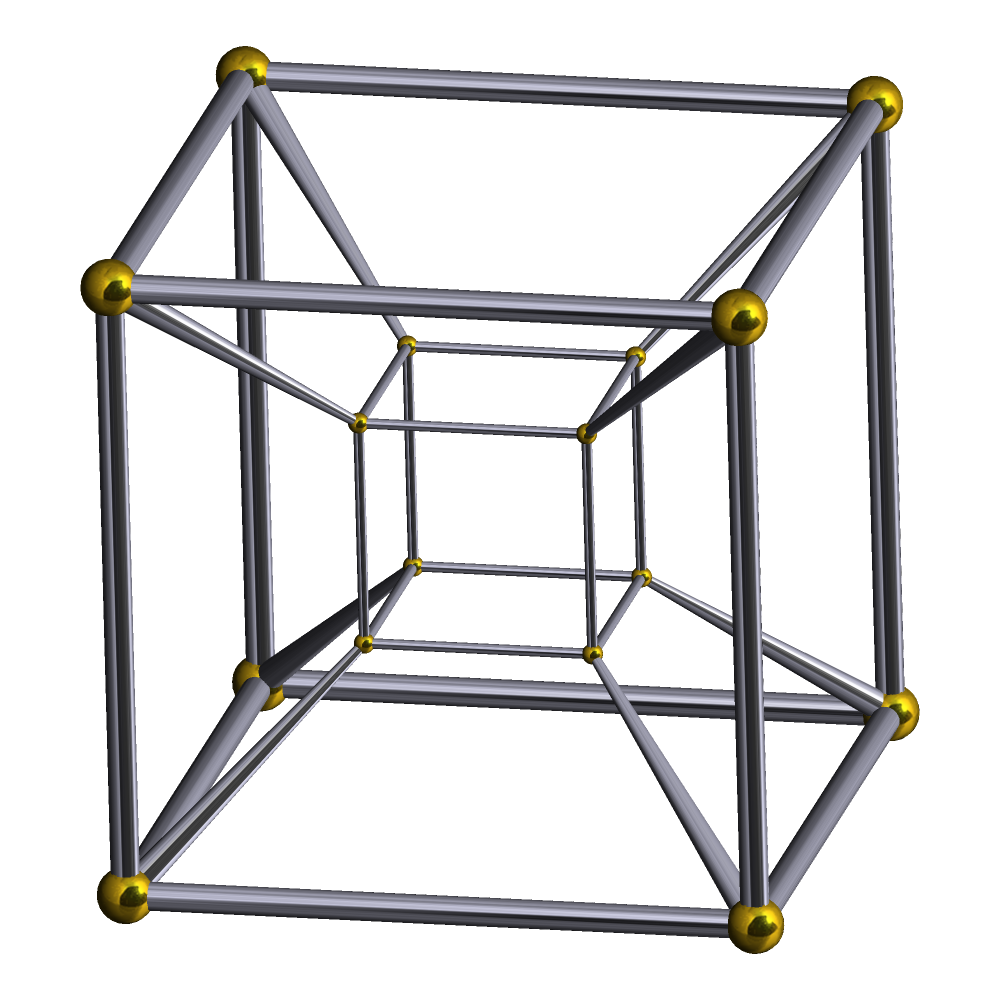
\includegraphics[width=1\textwidth]{hyper-cube.png}
    \caption{4х-мерный гиперкуб или тессеракт = $1^4$}
\end{figure}

\begin{figure}[H]
    \centering
    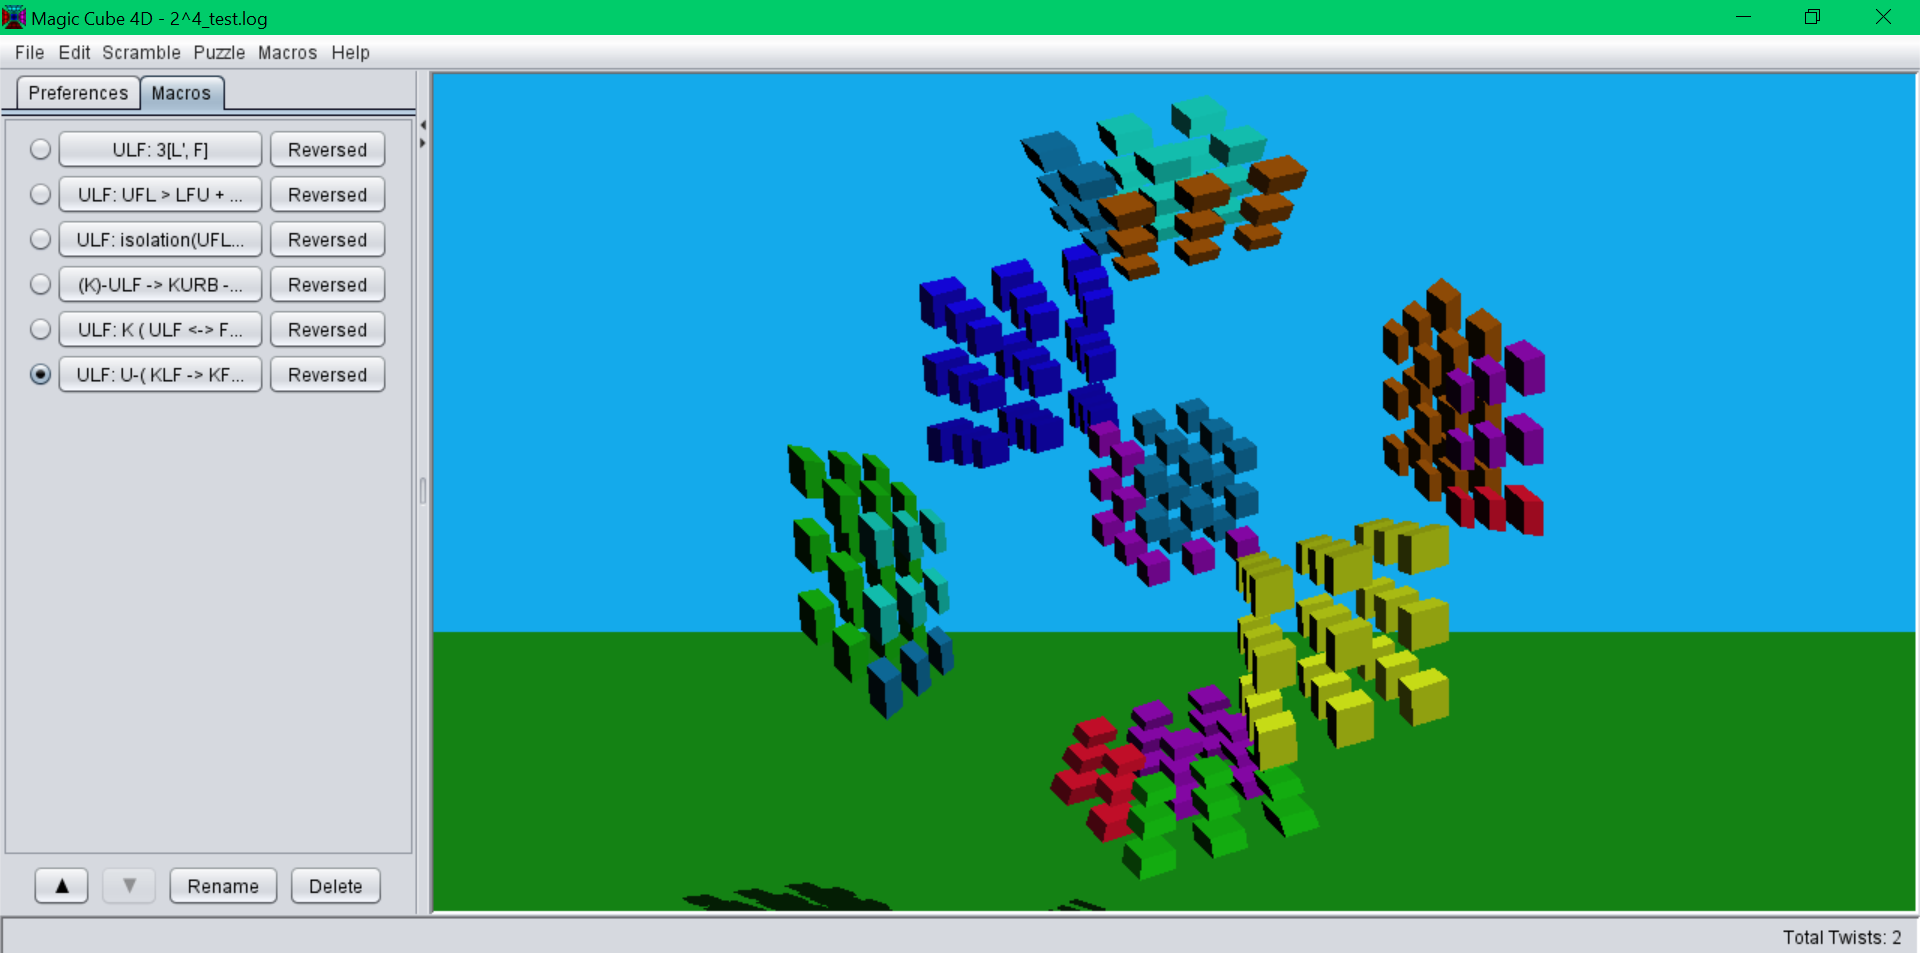
\includegraphics[width=1\textwidth]{3^4.png}
    \caption{4х-мерный гиперкубик Рубика 3х3х3х3 = $3^4$ (два поворота от собренного состояния)}
\end{figure}

\begin{figure}[H]
    \centering
    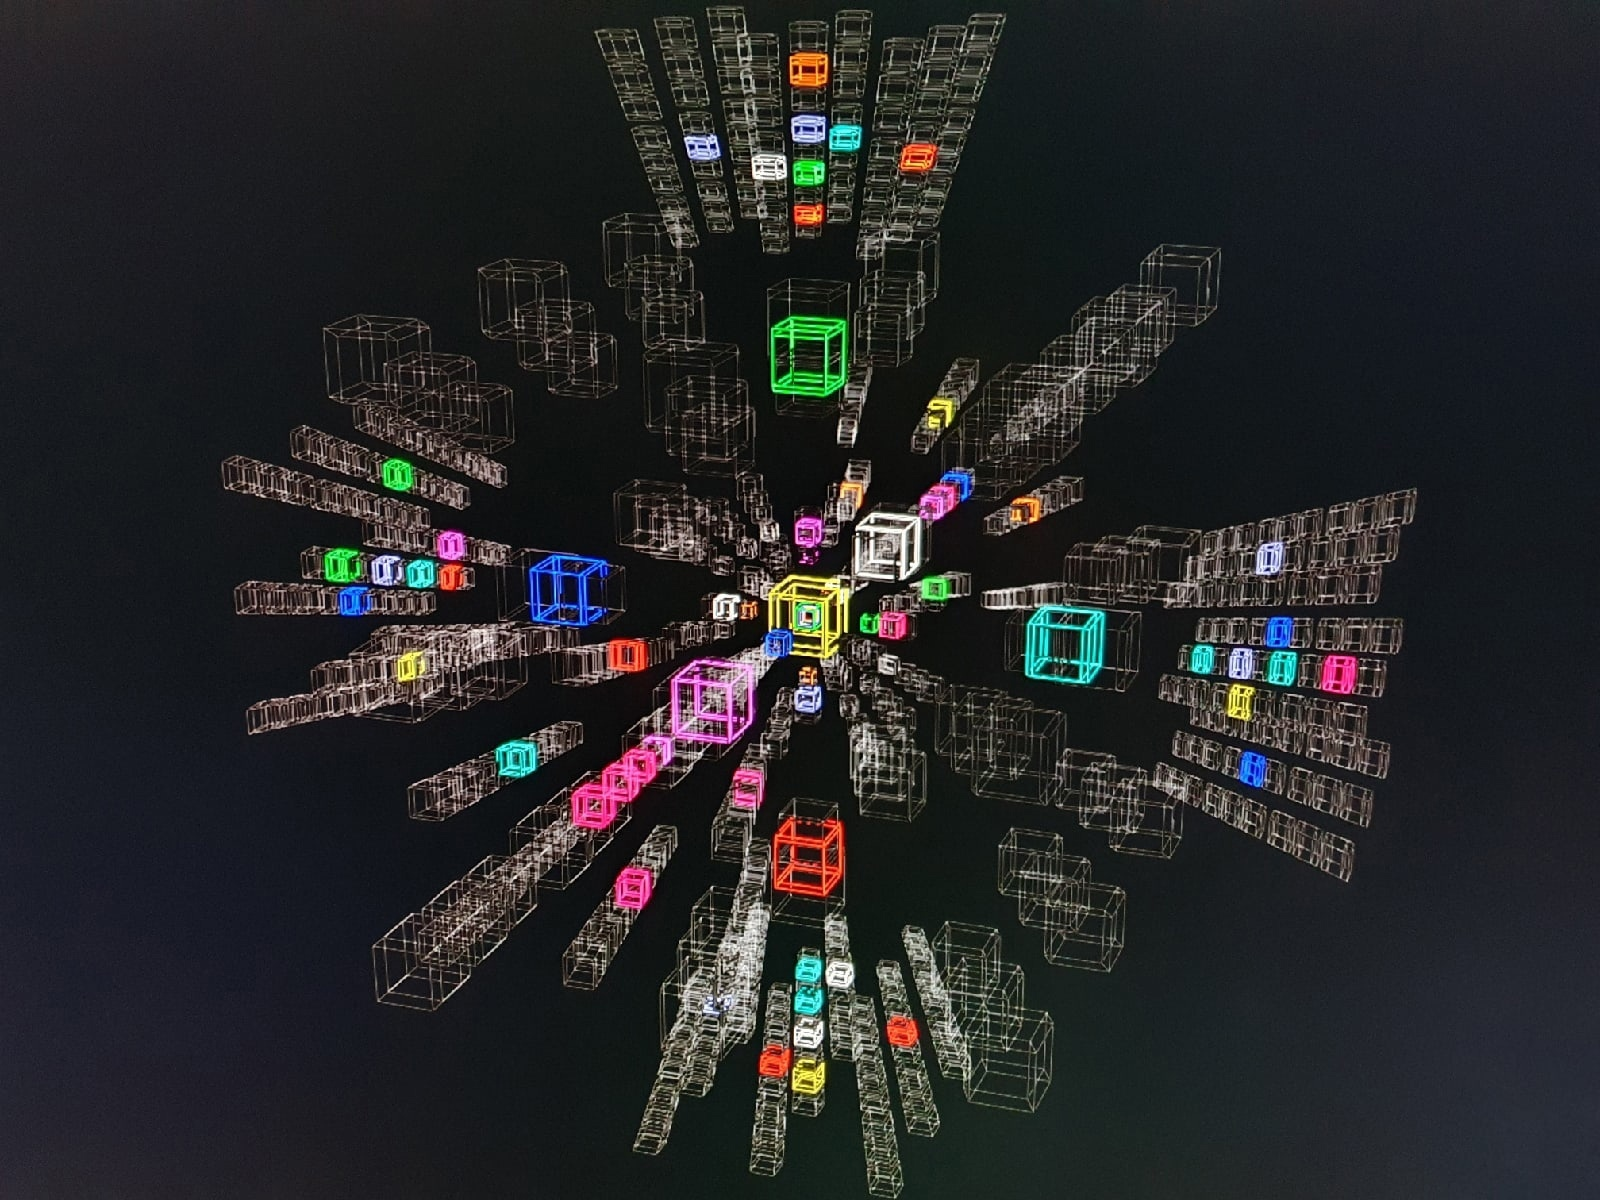
\includegraphics[width=1\textwidth]{5.jpg}
    \caption{5ти-мерный гиперкубик Рубика 3х3х3х3х3 = $3^5$}
\end{figure}

\begin{figure}[H]
    \centering
    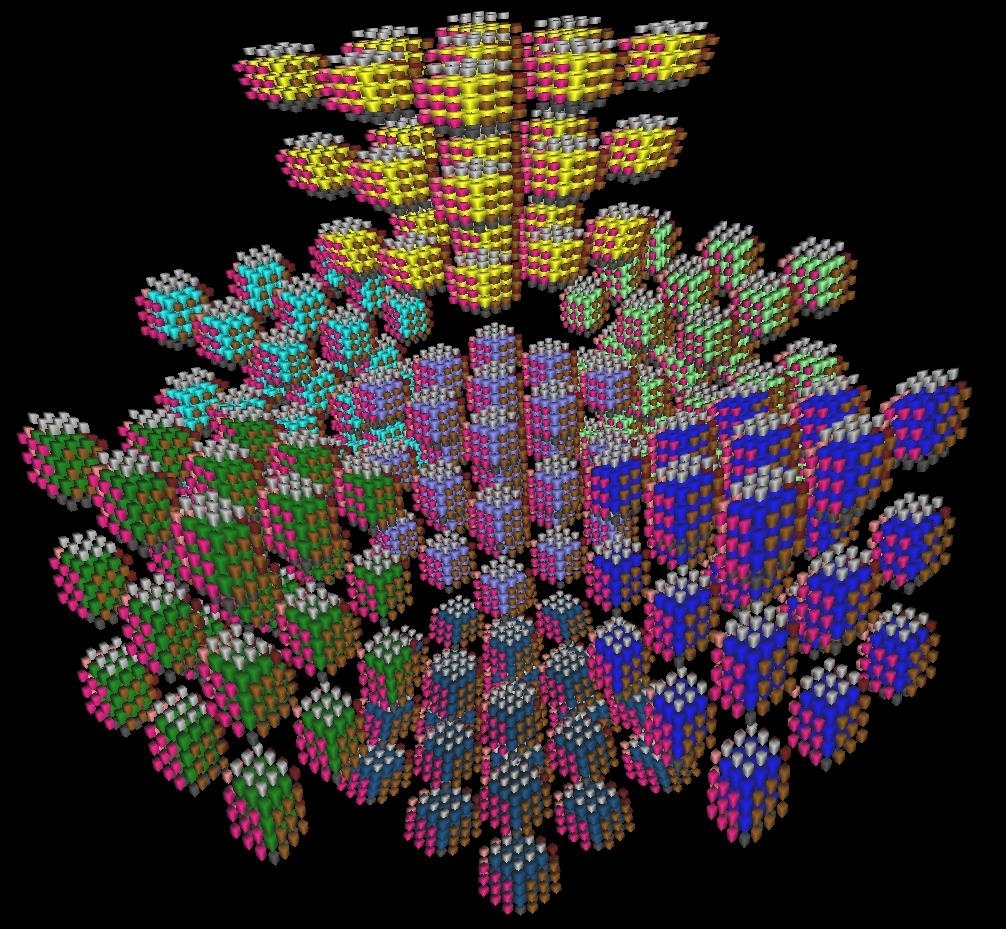
\includegraphics[width=1\textwidth]{7.jpg}
    \caption{7ми-мерный гиперкубик Рубика 3х3х3х3х3х3х3 = $3^7$}
\end{figure}

\begin{figure}[H]
    \centering
    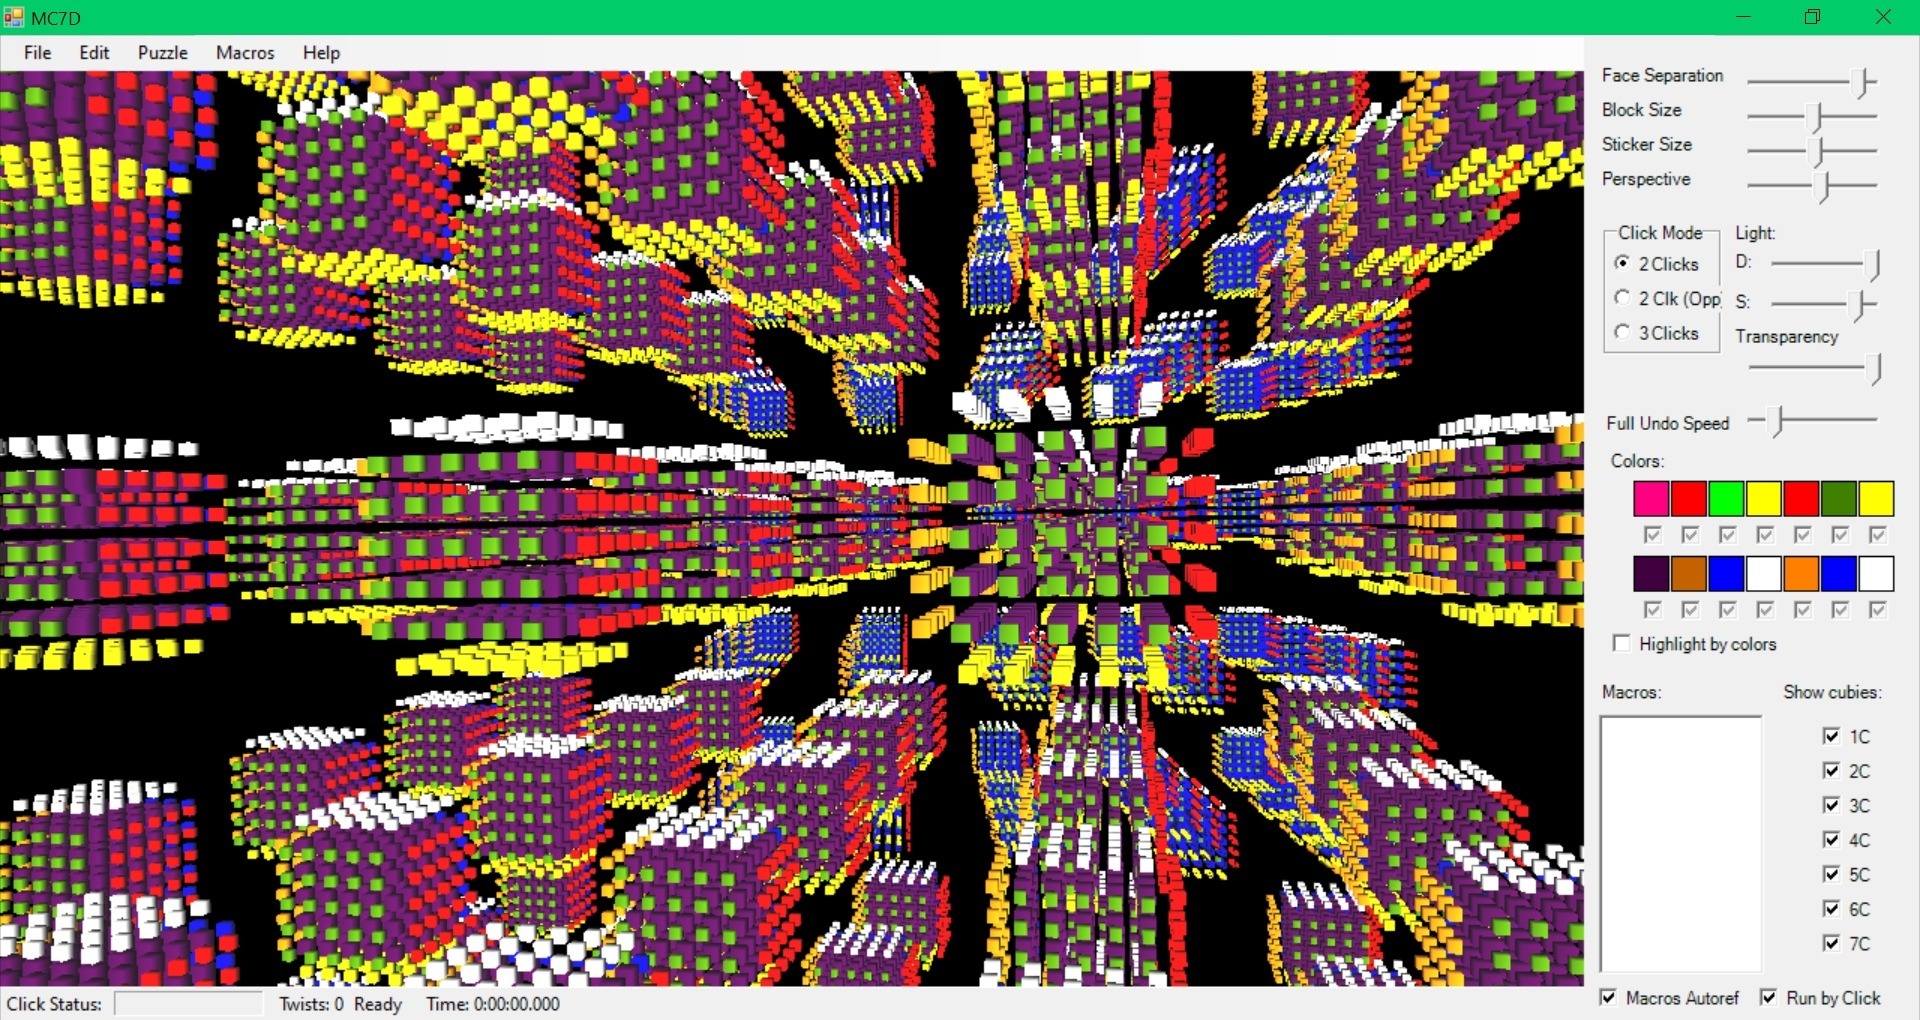
\includegraphics[width=1\textwidth]{7-2.jpg}
    \caption{7ми-мерный гиперкубик Рубика 3х3х3х3х3х3х3 = $3^7$}
\end{figure}

\begin{figure}[H]
    \centering
    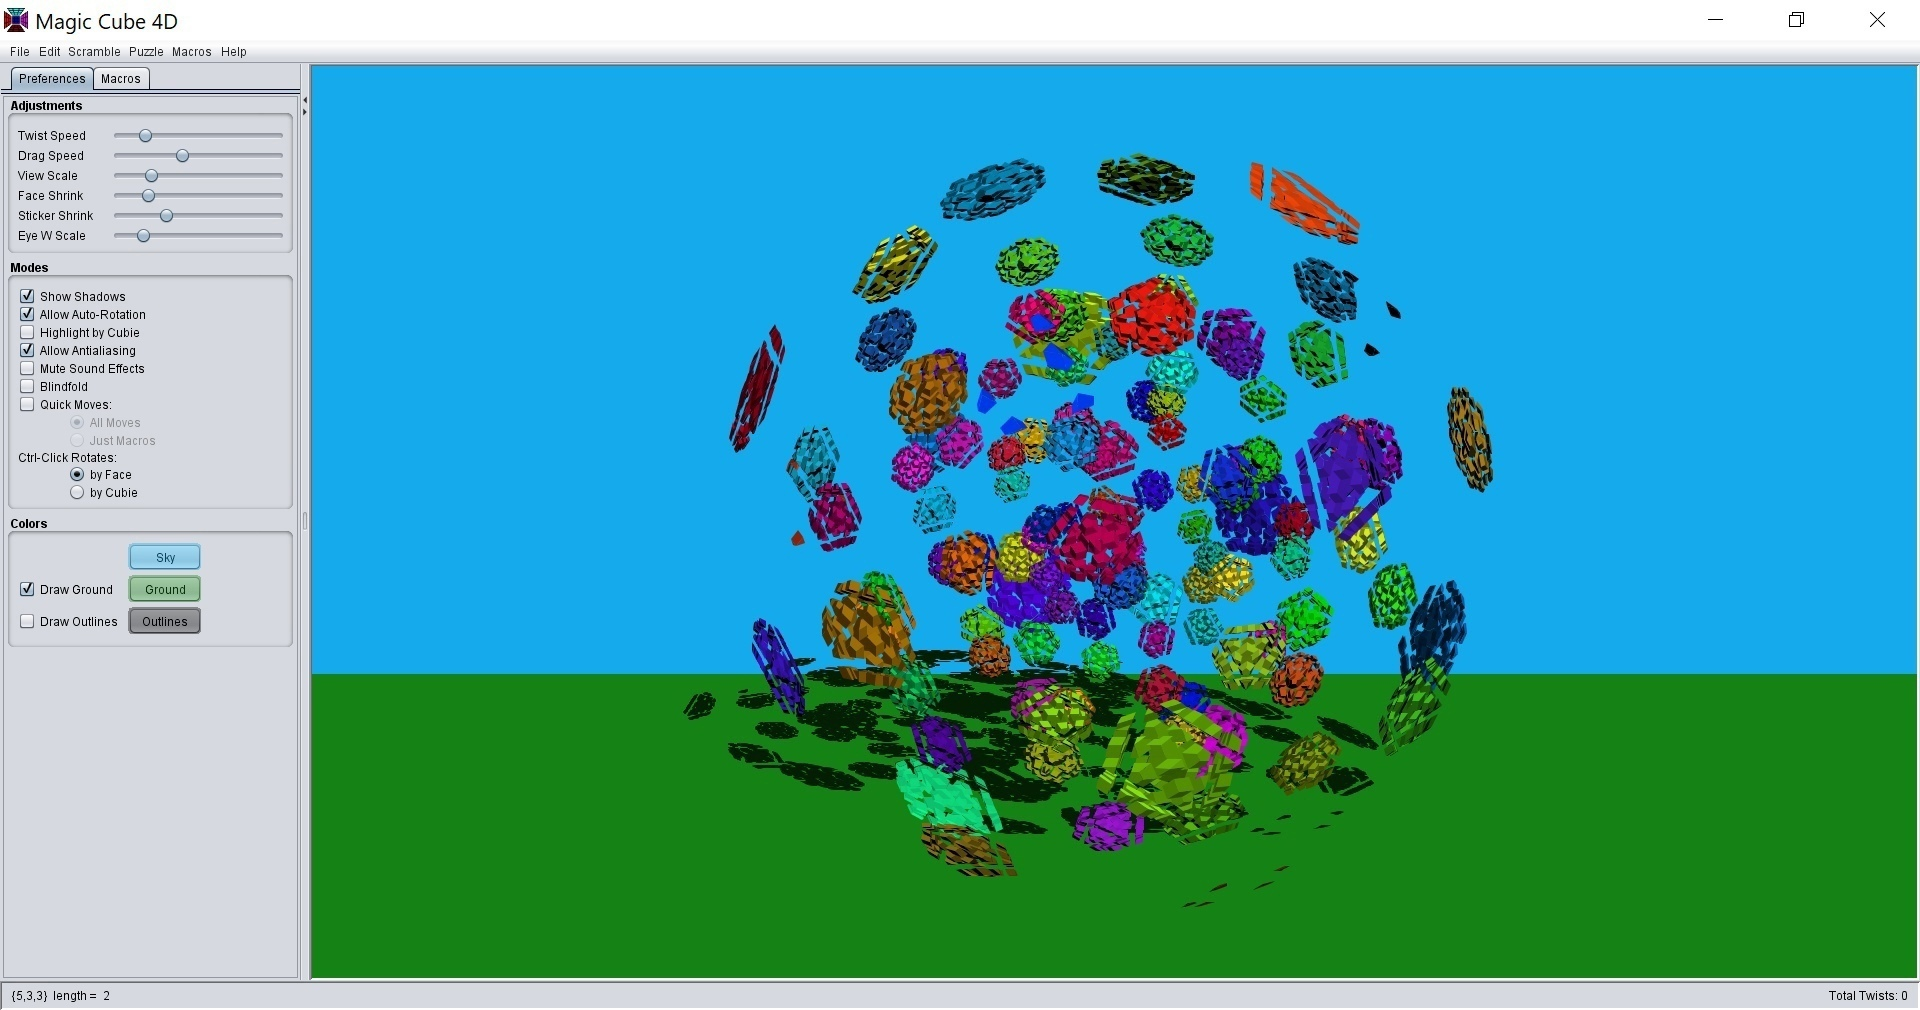
\includegraphics[width=1\textwidth]{120solved.jpg}
    \caption{120-ячейник Рубика (аналог додекаэдра в 4д)}
\end{figure}

\begin{figure}[H]
    \centering
    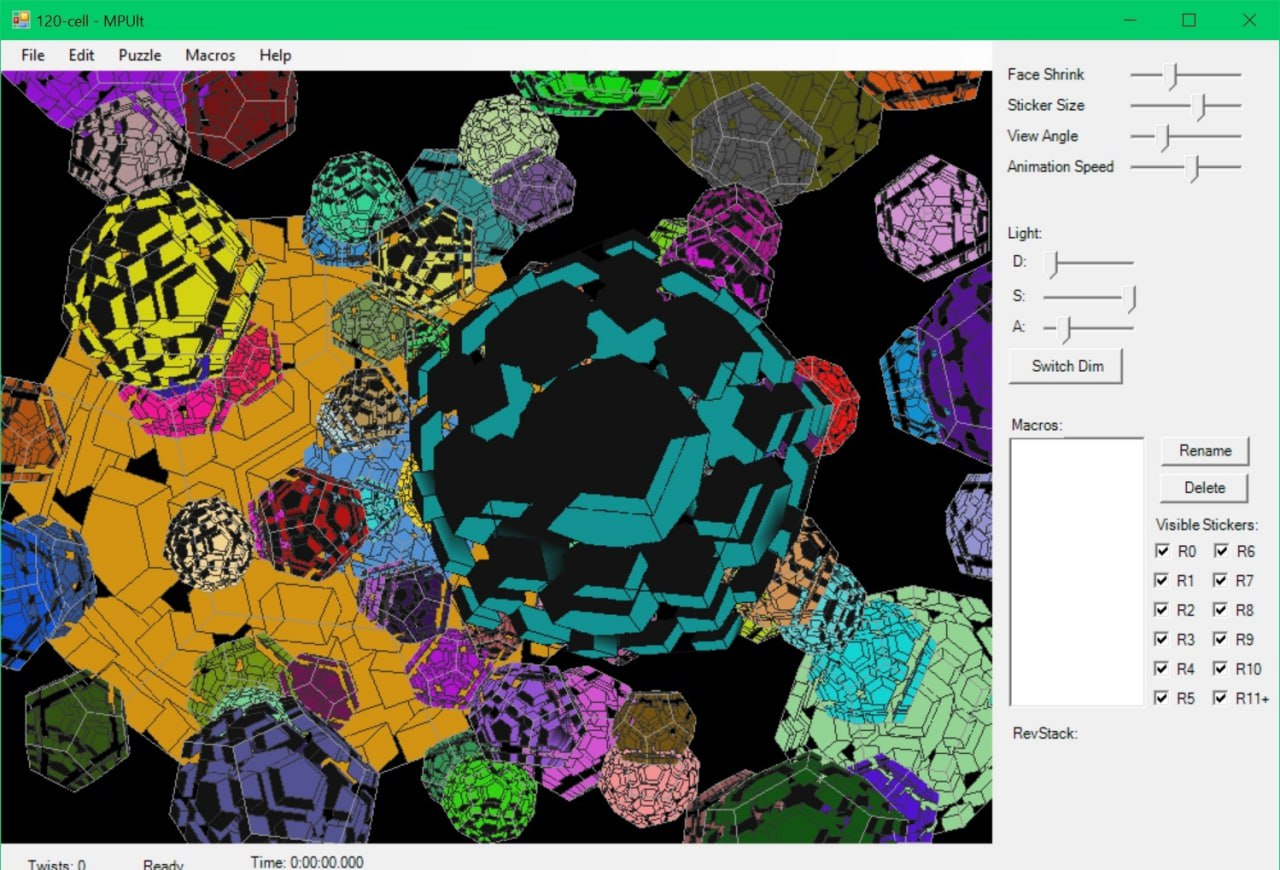
\includegraphics[width=1\textwidth]{120-2.jpg}
    \caption{120-ячейник Рубика (аналог додекаэдра в 4д)}
\end{figure}

\begin{figure}[H]
    \centering
    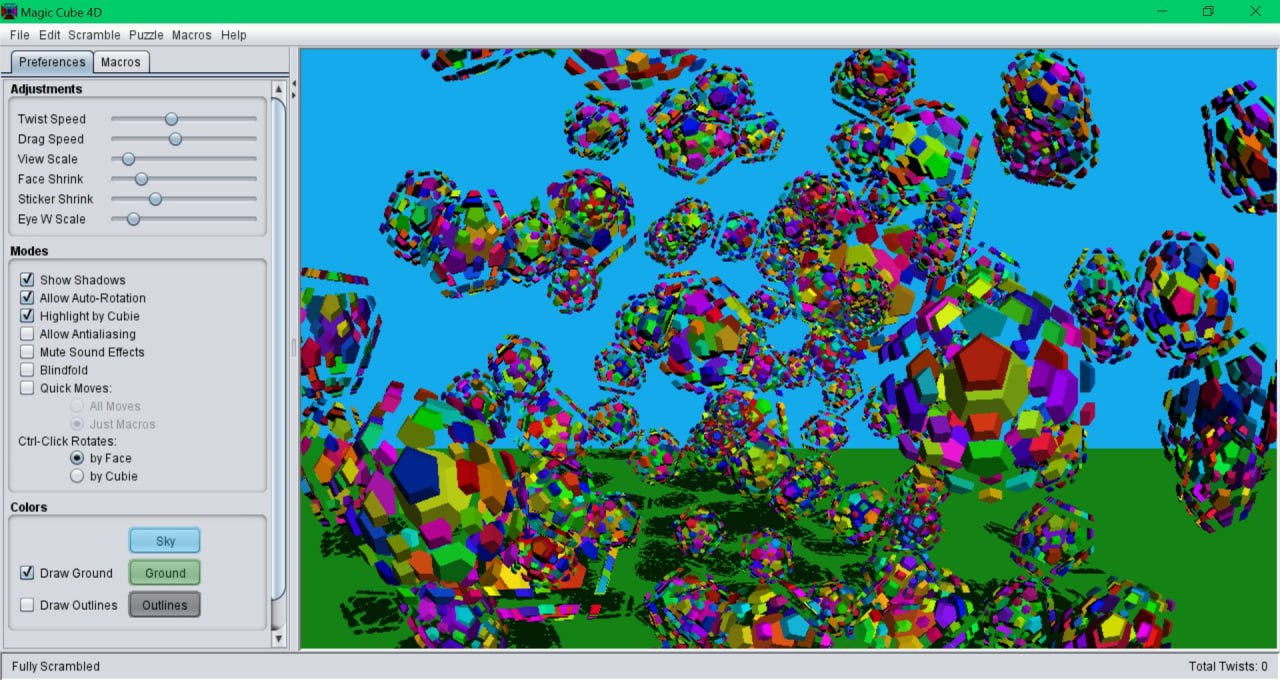
\includegraphics[width=1\textwidth]{120-3.jpg}
    \caption{120-ячейник Рубика (аналог додекаэдра в 4д), разобранный}
\end{figure}

\begin{figure}[H]
    \centering
    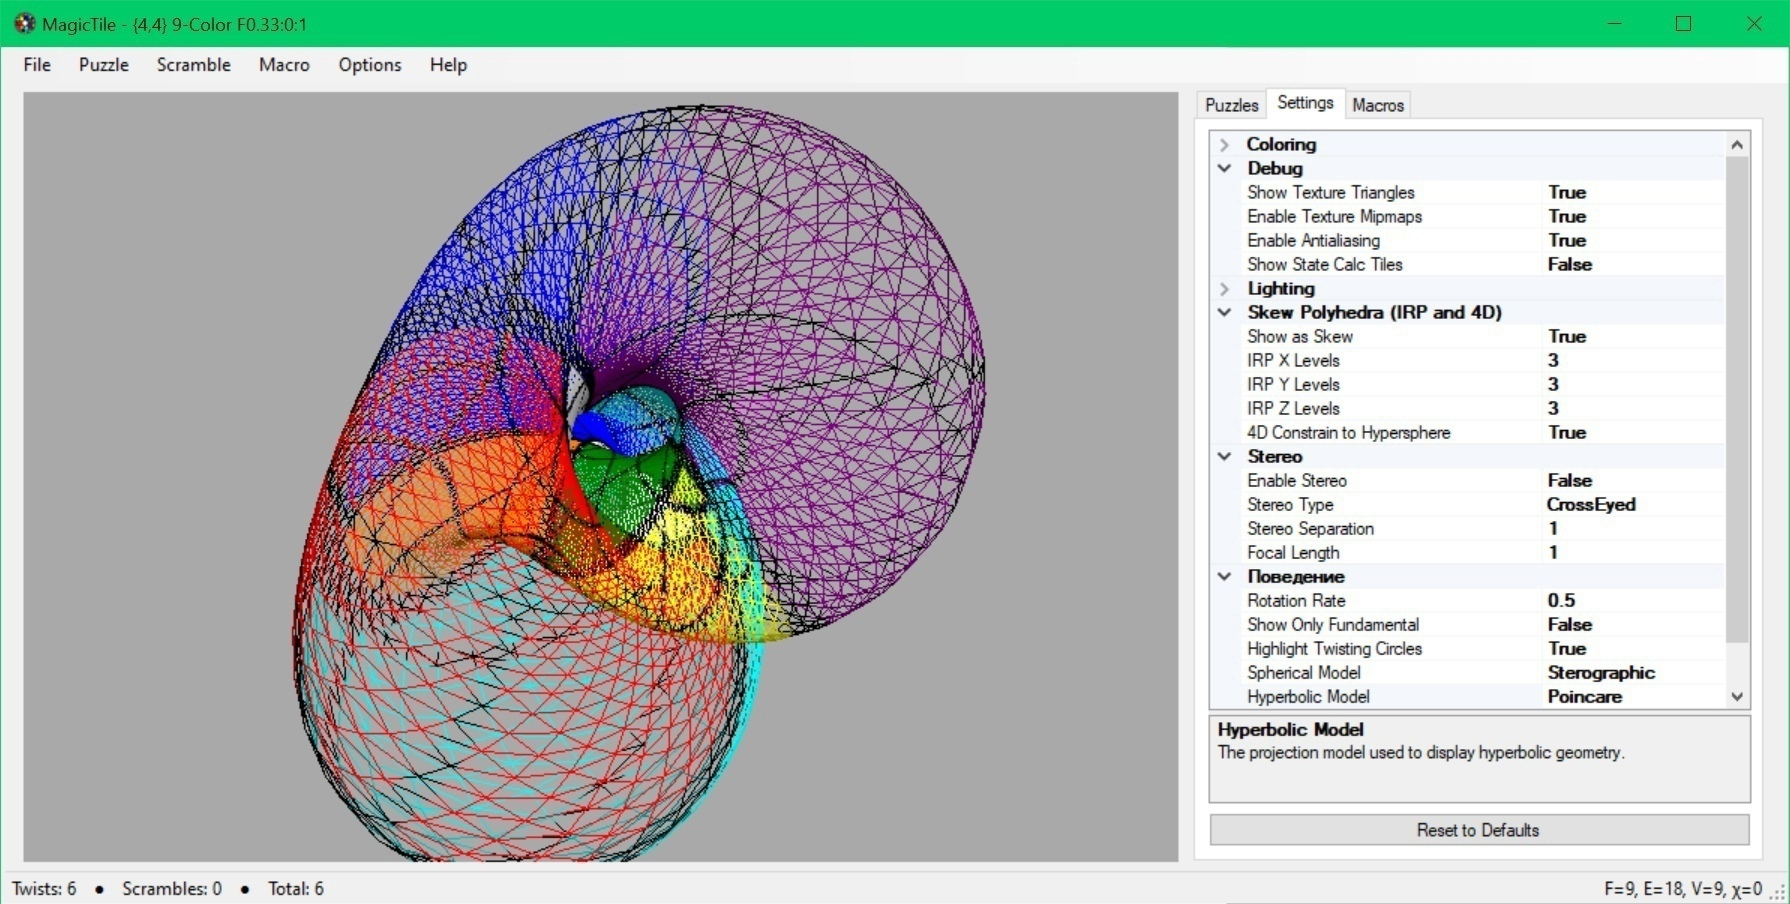
\includegraphics[width=1\textwidth]{Cline.jpg}
    \caption{Бутылка Клейна-Рубика}
\end{figure}

Сразу оговорюсь, что к самому Эрнё Рубику эти головоломки непосредственного отношения уже не имеют, и носят его имя чисто из дани уважения перед первопроходцем.

И еще одна оговорка: мне гораздо проще представлять себе пространство, будь оно хотя бы даже и 4D, без привязки к форме выражения. Это значит, что, если на соревнованиях по скоростной сборке кубика Рубика для дисциплины `Блаинд' (сборка с завязанными глазами) методы предполагают запоминание цветов мнемонически через ассоциацию с предметом, начинающимся на ту же букву, что и цвет (запоминается последовательность предметов), то мне гораздо проще представлять `голое пространство', а ассоциации и даже называние цветов меня наоборот лишь сбивают. Я прекрасно понимаю, что для объяснений какую-либо форму выражения все же придется выбрать и постараюсь сделать все возможное для ясного изложения. Поэтому же на своем канале AndyKybik я всегда называю цвета каждого элемента пазла, о котором говорю. Но когда речь идет о подготовке к ролику, я позволяю себе забыть на время о том, что кому-то что-то надо будет объяснять.

Так например, мне удалось \textbf{устно!} просчитать наперед \textbf{161, Карл!, поворот} на кубике \textbf{со склеенными элементами!}. После чего я дважды все проверил по памяти и все срослось. Собственно, вот его схема:

\begin{figure}[H]
    \centering
    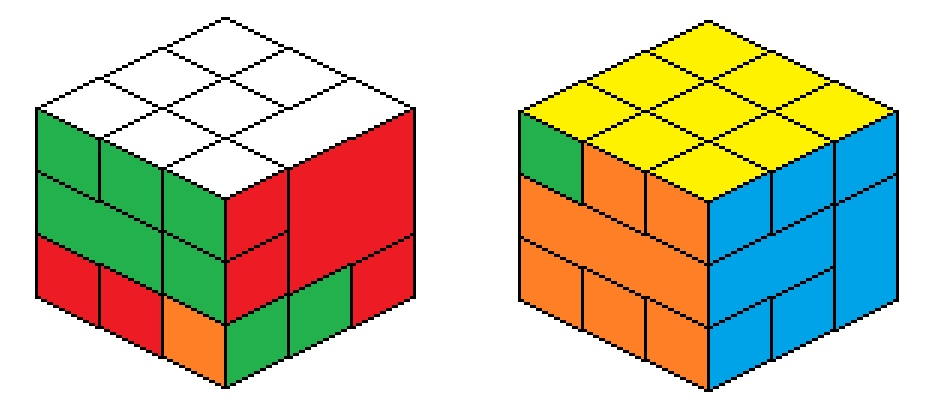
\includegraphics[width=1\textwidth]{evil_bandage.jpg}
    \caption{Один из самх злых бандажей, которые мне доводилось решать (если не самый злой вообще, во всяком случае для 3х3х3). Бандаж - куб/пазл иной формы со склеенными элементами или другими - более сложными и хитрыми, необычными ограничениями. Строго говоря, типов этих ограничений столько же, сколько и куберов, их выдумывающих.}
\end{figure}

}

\chapter{Комбинаторика}

Мы коснемся разных задач, но сначала мы (как и я в свое время) будем подходить к ним со школьной комбинаторной позиции. И лишь главах далее мы дадим определения группе и морфизмам, через которые данные задачи решатся в один шаг. Я бы мог дать их сразу, но, чтобы прочувствовать силу инструмента, надо, как это говорят бизнесмены, `пройти через личную боль'.

Чтобы было понятно, о чем речь, задачи, которых мы коснемся, могут звучать как-то так: \\

\begin{enumerate}
\item \textit{Найти общую формулу подсчета числа ориентаций у куба размерности N.}
\item \textit{Найти общую формулу подсчета числа ребер и Платонова Тела в 3д, имея информацию и очисле его граней и числе углов на каждой из них.}
\end{enumerate}

Но для того, чтобы научиться считать такие вещи, пускай и на школьном уровне, необходимо знать комбинаторные функции: $C_n^k$ (биномиальный коэффициент, сочетания), $A_n^m$ (перестановки) и $P_n$ (размещения). Но вместо того, чтобы давать здесь определения этих формул и сразу сухие классические упражнения, оставляющие вопросы у начинающих, как и когда их применять, я дам их вывод. Ведь во всяком случае я всегда мыслил связями, и запомнить причину мне всегда было проще, чем запомнить ничем не подкрепленное `абстрактное следствие в вакууме' (напоминаю, что этот документ - все еще мой конспект).

\section{Вывод формул}

\section{Упражнения}

\chapter{Типы многограников (трехмерное пространство)}

\section{Архимедовы, Платоновы и Каталановы тела, число в каждом виде, примеры, картинки}

\section{Комбинаторика трехмерных многогранников}

\begin{enumerate}
\item \textit{Число углов и ребер у трехмерного платонова тела по числу граней и углов на каждой}

\item \textit{Число углов, ребер, граней, гиперграней у гипер-куба любой мерности (вывод формулы: рекуррентной - эмпирически и эффективной - доказательно)} 
\end{enumerate}

Позже коснемся этого раздела с точки зрения Теории Групп.

\section{Упражнения}

Подстановка фигур в формулы и сверка резульатов.

\chapter{Преобразования пространства и их определения}

\section{Базовые определения (Теория Множеств)}


Перед тем как перейти к терминам, имеющим отношение к перемещениям в пространтсве, полезно уточнить несколько фундаментальных понятий, часто используемых в алгебре, логике и теории множеств. Понятия в данном разделе даны в порядке увеличения связей, однако в примерах может быть некоторая непоследовательность применения обозначений этих терминов.\\

\textbf{Связь элементов во множествах:}

\begin{enumerate}[label=\arabic*., parsep=4pt, itemsep=4pt, topsep=4pt, partopsep=0pt]

\item \textbf{Неупорядоченная пара $\{a,b\}$} - пара любых элементов (в том числе других неупорядоченных пар), в которой их порядок не важен.

$(a,b) = (b,a)$ (даже при $a \neq b$)

\item \textbf{Упорядоченная пара $(a,b)$} - пара любых элементов (в том числе других пар, как упорядоченных, так и нет), в которой порядок учитывается.

$(a,b) \neq (b,a), a \neq b$

\item \textbf{Свойства Упорядоченных и Неупорядоченных пар:}

Любые две упорядоченные пары, отличающиеся лишь порядком следования объектов, дают одну и ту же неупорядоченную пару.
Иными словами, пара векторов $\{\overrightarrow{v_1}, \overrightarrow{v_2}\}$ может быть сложена из $(\overrightarrow{v_1}, \overrightarrow{v_2})$ и $(\overrightarrow{v_2}, \overrightarrow{v_1})$.

\textbf{ПРИМЕРЫ ЧЕРЕЗ ЛИНЕЙНЫЕ И НЕЛИНЕЙНЫЕ КОМБИНАЦИИ}

\item \textbf{Отношение (n-арное отношение)} - подмножество декартова произведения множеств.

Пусть даны $A_1, A_2, ... , A_n$. Тогда $n-$арное отношение $R$ - это любое подмножество их декартова произведения:

$R \subseteq A_1 \times A_2 \times \ldots \times A_n$

При $n = 2$ $R -$ бинарное отношение.\\
При $n = 3$ $R -$ тернарное отношение.\\
При $n = 4$ $R -$ тетрарное отношение.\\
И т.д. (можно представить как ячейки гипер-куба/кубоида)

\textbf{Пример:}

Бинарное отношение «меньше» на $\mathbb{N}: R = {(a,b) | a<b} \subset \mathbb{N} \times \mathbb{N}:$

\begin{figure}[H]
\centering
\begin{tikzpicture}[scale=0.8, thick]

% Оси
\draw[->] (0,0) -- (6.5,0) node[right] {$a$};
\draw[->] (0,0) -- (0,6.5) node[above] {$b$};

% Сетка
\draw[gray!30, very thin] (0,0) grid (6,6);

% Диагональ y = x
\draw[dashed, gray, thick] (0,0) -- (6,6) node[midway, above left, black] {$b = a$};

% Закрашенная область: b > a (выше диагонали)
\fill[blue!20, opacity=0.5] (0,0) -- (0,6) -- (6,6) -- cycle;

% Метки на осях
\foreach \i in {1,...,6} {
    \draw (\i,0.1) -- (\i,-0.1) node[below] {\tiny $\i$};
    \draw (0.1,\i) -- (-0.1,\i) node[left] {\tiny $\i$};
}

% Подпись: отношение a < b
\node at (3,1.5) [text=black, opacity=0.7] {\large $a < b$};
\node at (1.5,3) [text=blue, opacity=0.7, font=\small, align=center] at (2.5,4.5) {область\\отношения};

\end{tikzpicture}
\caption{Графическое представление отношения $a < b$, $a, b \in \mathbb{N}$}
\label{fig:relation-a-less-b}
\end{figure}

\begin{figure}[H]
\centering
\tdplotsetmaincoords{60}{120} % Углы обзора: камера сверху слева
\begin{tikzpicture}[tdplot_main_coords, scale=1.2, thick]
% Оси
\draw[->] (0,0,0) -- (5,0,0) node[right] {$x$};
\draw[->] (0,0,0) -- (0,5,0) node[above right] {$y$};
\draw[->] (0,0,0) -- (0,0,4) node[above] {$z$};
% Сетка (опционально)
\foreach \i in {1,...,4} {
    \draw[gray!30, very thin] (\i,0,0) -- (\i,5,0);
    \draw[gray!30, very thin] (0,\i,0) -- (5,\i,0);
    \draw[gray!30, very thin] (0,0,\i) -- (5,0,\i);
    \draw[gray!30, very thin] (0,0,\i) -- (0,5,\i);
}
% Плоскость z = y - x (граница)
% Рисуем поверхность z = y - x в пределах [0,4] для x,y
% Используем сетку из линий
\foreach \u in {0,0.5,...,4} {
    \draw[blue!50, thin] plot[domain=\u:4, variable=\v] ({\u}, {\v}, {\v-\u});
}
\foreach \v in {0,0.5,...,4} {
    \draw[blue!50, thin] plot[domain=0:\v, variable=\u] ({\u}, {\v}, {\v-\u});
}
% --- НОВОЕ: Треугольник в плоскости y=4 ---
% Границы: z=4 (x от 0 до 4), x=4 (z от 0 до 4), x=4-z (от (4,0) до (0,4))
% Сетка треугольника: линии параллельные x (при фиксированном z)
\foreach \z in {0,0.5,...,4} {
    % Рисуем линии от x=0 до x=4-z (ограничены треугольником)
    \draw[blue!50, thin] plot[domain=0:{4-\z}, variable=\x] ({\x}, {4}, {\z});
}
% Сетка треугольника: линии параллельные z (при фиксированном x)
\foreach \x in {0,0.5,...,4} {
    % Рисуем линии от z=0 до z=4-x (ограничены треугольником)
    \draw[blue!50, thin] plot[domain=0:{4-\x}, variable=\z] ({\x}, {4}, {\z});
}
% --- Конец нового ---
% Подпись: отношение z < y - x
% ИЗМЕНЕНО: Перенесено левее и ниже, шрифт увеличен, добавлено align=center
\node at (2, 2.5, 0.5) [text=black, opacity=0.8, font=\small, align=center] {$z < y - x$}; % <-- Изменено положение и размер
% Метки на осях
\foreach \i in {1,...,4} {
    \draw (\i,0.1,0) -- (\i,-0.1,0) node[below] {\small $\i$}; % <-- Изменено: \tiny -> \small
    \draw (0.1,\i,0) -- (-0.1,\i,0) node[left] {\small $\i$}; % <-- Изменено: \tiny -> \small
    \draw (0,0.1,\i) -- (0,-0.1,\i) node[left] {\small $\i$}; % <-- Изменено: \tiny -> \small
}
% Подпись области
\node at (2, 3, 2.5) [text=blue, opacity=0.7, font=\footnotesize, align=center] {область\\отношения};
\end{tikzpicture}
\caption{Графическое представление отношения $z < y - x$, $x, y, z \geq 0$}
\label{fig:relation-z-less-y-minus-x}
\end{figure}

\item \textbf{Соответствие между множествами $A$ и $B$} - это тройка $(A, B, R)$, где $R \subseteq A \times B$ - бинарное отношение. Элемент $a \in A$ соответствует элементу $b \in B$, если $(a,b) \in R$. Термин «соответствие» подчёркивает направленность связи между двумя множествами. Он часто используется как синоним бинарного отношения, когда важно явно указать \textit{исходное} и \textit{целевое} множество.

\end{enumerate}

$ $\\

\textbf{Типы множеств:}\\

\begin{enumerate}[label=\arabic*., parsep=4pt, itemsep=4pt, topsep=4pt, partopsep=0pt]

\item \textbf{частично упорядоченное множество (ЧУМ, англ. poset) $(X, \leqslant)$} - множество $X$, для которого соблюдаются:

\begin{enumerate}[label=\arabic*., parsep=4pt, itemsep=4pt, topsep=4pt, partopsep=0pt]

\item \textbf{Рефлексивность:} $\forall x \in X, x \leqslant x$ 

Формально, отношение $R$ на множестве $A$ называется рефлексивным, если для всех элементов $a$ из $A$ пара $(a, a)$ является частью отношения $R$:

$R \subseteq A_1 \times A_2 \times \ldots \times A_n$
$a \in A: (a,a) \in R$

Некоторые примеры рефлексивных отношений:

\begin{enumerate}[label=\arabic*., parsep=4pt, itemsep=4pt, topsep=4pt, partopsep=0pt]

\item Равенство. Отношение равенства на любом множестве является рефлексивным, так как каждый элемент равен самому себе.

\item «Является кратным». На множестве целых чисел отношение «является кратным» рефлексивно, потому что каждое целое число является кратным самому себе.

\item «Является подмножеством». На множестве всех множеств отношение «является подмножеством» рефлексивно, так как каждое множество является подмножеством самого себя.

\item «Является конгруэнтным по модулю n». На множестве целых чисел отношение «является конгруэнтным по модулю n» рефлексивно, потому что каждое целое число конгруэнтно самому себе по модулю любого целого числа n.

\end{enumerate}

\item \textbf{Антисимметричность:}

\item \textbf{Транзитивность:}

\end{enumerate}

\item \textbf{Линейно упорядоченное множество} - ???

\item \textbf{Вполне упорядоченное множество} - ???

\item \textbf{Плотное множество} - ???

\item \textbf{Направленное множество} - ???

\item \textbf{Решётка} - частично упорядоченное множество, в котором каждое двухэлементное подмножество имеет как \textbf{точную верхнюю}, так и \textbf{точную нижнюю грани}.

\textbf{ПРИМЕРЫ}

\end{enumerate}

$ $\\

Теперь же дадим определения \textbf{связям между множествами}:

\begin{enumerate}[label=\arabic*., parsep=4pt, itemsep=4pt, topsep=4pt, partopsep=0pt]

\item \textbf{Отображение (Mapping)} — любое правило, которое сопоставляет каждому элементу одного множества некоторый единственный элемент другого. \\

$f: A \to B, f \subset A \times  B $ \\
$\forall a \in  A \exists ! b \in B: (a,b) \in f$ \\

Читаем: $f$ — это \textit{отображение} из $A$ в $B$ такое, что $f$ — это подмножество декартова произведения $A$ и $B$. Например, легко это визуально представить как табличку (конечную или бесконечную), прямоугольник на координатной плоскости или же саму эту плоскость. И мы выбираем такие их ячейки/точки, что каждой ячейке/точке из $A$ (каждой координате $x$) соответствует единственная ячейка/точка из $B$ (координата $y$), и пара этих соответствующих друг другу элементов принадлежит $f$.\\

\item \textbf{Функция (Function)} — это отображение, у которого \textit{область определения} (подмножество исходного множества $A$, с каковым подмножеством мы работаем) совпадает с исходным множеством (то есть определена всюду).  

Например, если $A = \{1,2,3\}, A' = \{1,3\}, B = \{a,b\}$, где $A$ - иходное мноежтсво, из которого работает фукнция $f$, $A' \subset A$ - подмножество $A$, то есть область определения $f$, $B$ - итоговое множество, внутрь которого работает $f$, то \\

$f(x): \left\{ \begin{matrix} 
a, x = 1 \\
b, x = 3
\end{matrix} \right.$ \\

-- это функция, а \\

$f(x) = \left\{ a, x = 3\right.$ \\

-- это НЕ функция. \\

Спор о разнице между отображением и функцией можно вести долго. В конце концов, категоризация исторически сложившихся концепций и сущностей — крайне неблагодарное занятие, что известно мне очень хорошо еще из кубинга — я пытался создать максимально общую модель головоломок, и так и не смог сделать это до конца. Ирония в том, что моя модель была геометрической, а на деле она должна было быть чем-то вроде Группы, к чему мы и подойдем.  

Исторически \textit{отображение} было чем-то более общим, и могло, вероятно, работать не на всей области определения. Однако в современных материалах эти слова — скорее синонимы. Иногда под \textit{отображением} подразумевается все еще нечто более широкое по сравнению с \textit{функцией}. Но и тут могут быть исключения:

\end{enumerate}

\begin{enumerate}[label=\arabic*., parsep=4pt, itemsep=4pt, topsep=4pt, partopsep=0pt]

\item Функция арифметического (не комплесного) корня - технически, если подходить к вопросу со всей строгой историчской педантичностью, это скорее \textit{отображение}, так как область определения $\ge 0$, то есть $[0, +\infty)$, а не $(-\infty, +\infty)$. Но все привыкли говорить `функция корня'.

\item Функции, имеющие точки разрыва, где их значение не определено или является $+\infty$ или $-\infty$. Примерами таких функций могут служить $y = 1/x$ или $y = tg(\alpha)$

\end{enumerate}

Условно говоря, можно провести следующую аналогию: отображение - это проекция куба размерности $N>M$ в размерность $M<N$ (то есть вниз). При проецировании некоторые вершины, ребра, гиперграни или другие составляющие могут наложиться друг на друга и слиться. В этом случае сам исходный образ гипер-куба несет в себе больше информации, чем его проекция. Функция же в таком случае - это развертка куба. В развертке нет потери информации, и, я бы сказал, она несет даже больше информации, чем исходный образ, так как некоторые вершины и ребра повторяются дважды и трижды в рамках самой развертки (попробуйте мысленно-визуально проассциировать вершины развертки куба 3д и его самого?)

\textbf{Упражнение}

Являеются ли исключением функции:

\begin{enumerate}[label=\arabic*., parsep=4pt, itemsep=4pt, topsep=4pt, partopsep=0pt]

\item Дирихле: всюду разрывна, но определена - равна 1, если аргумент рационален, и 0, если иррационален\\

$f: \left\{ \begin{matrix} 
1, x \in &\mathbb{Q}\\
0, x \in &\mathbb{R}\textbackslash\mathbb{Q}
\end{matrix} \right.$ \\

(Ответ: нет, функция Дирихле действует на всей области определения)

\item Вейерштрасса - непрерывна, но нигде не дифференцируема (изломана в каждой точке, как $|x|$ в $x=0$). \\

$w(x) = \sum_{n=0}^{\infty} b^n \cdot cos(a^n \pi x), f: \left\{ \begin{matrix} 
a \in \mathbb{N}, a \nmid 2 \\
b \in (0,1)
\end{matrix} \right.$ \\

\begin{minipage}[t]{\linewidth}
    \centering
    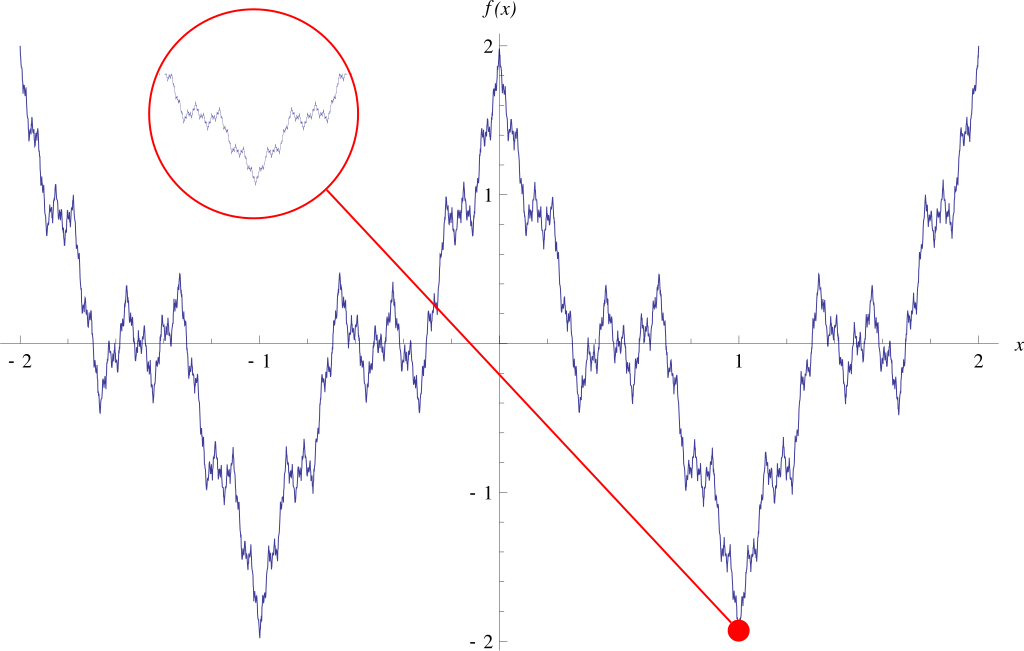
\includegraphics[width=0.8\textwidth]{Вейерштрасс.png}
    \captionof{figure}{Фрактальная всюду изломанная, но непрерывная функция Вейерштрасса}
\end{minipage}

(Ответ: нет, функция Вейерштрасса определена на всей области определения, на что прямо подсказывает фраза под картинкой)

\end{enumerate}

Свойства Функций: 

\begin{enumerate}[label=\arabic*., parsep=4pt, itemsep=4pt, topsep=4pt, partopsep=0pt]

\item Инъективность (вложение): функция $f: A \to B$ инъективна, если разные элементы из $A$ переходят в разные элементы из $B$.

$b_1 = f(a_1)$
$b_2 = f(a_2)$
$f(a_1) = f(a_2) \Rightarrow a_1 = a_2 \Leftrightarrow \forall b \in B: |\{a \in A | f(a)=b\}| \le 1$

Читаем: если образы равны, то и прообразы равны. Или: каждый элемент из $B$ имеет не более одного прообраза.

Это можно представить визуально, если поднимать по оси $y$ из $-\infty$ в $+\infty$ горизонтальную прямую и сверять, сколько точек лежит на этой прямой. Если на каждой прямой лежит только одна точка - функция инъективна. Если хотя бы на одной прямой более одного прообраза - то функция сразу не инъективна (проще говоря, для контраргумента ищем повторение по $x$).

Примеры строго инъективных функций (только свойство инъекции): $y = log(x)$, $y = exp(x)$ (не все $y$ покрыты, а только $y>0$, но каждому $x$ есть свой и только один $y$)

\item Сюръективность (покрытие): функция $f: A \to B$ сюръективна, если каждый элемент B имеет хотя бы один прообраз (задействована вся область значений, каждое по одному разу)

$\forall b \in B: |\{a \in A| f(a)=b\}| \ge 1$

Читаем: каждый элемент из $B$ имеет хотя бы один прообраз.

Это можно представить визуально, если вести по оси $y$ из $-\infty$ в $+\infty$ горизонтальную прямую и искать хотя бы одну точку на каждой прямой. Если на каждой прямой есть хотя бы одна точка (покрыты все $y$) - функция сюръективна. Если хотя бы на одной прямой нет точки, функция сразу не сюръективна (проще говоря, для контраргумента ищем пустоту по $y$).

Примеры строго сюръективных функций (только свойство сюръекции): $y = (\sum_{i=0}^{N}a_ix^i)+c, n > 2, a_i > 0$ (степенная функция с локальными минимумами и максимумами, то есть имеющая изгибы - покрыты все $y$, но некоторые из них встречаются $>1$ раза).

Если поменять местами $A$ и $B$ (поворот координатной плоскости вокруг диагонали $x=y$ или иначе -- обратное отображение, инверсия), инъекция имеет опасность перестать быть функцией -- ведь и правда $y = |x|$, положенный `на бок' ($x = |y|$) имеет не одно, а два значения везде, где $x>0$, равно, как и $y = sin(x) \longrightarrow x = sin(y)$ становится неоднозначной, как комплексный корень. Впрочем, не все функции имеют такую опасность: например $y=kx+b \longrightarrow x = \frac{y-b}{k}$ (наклон прямой на 90 градусов) не нарушает условия функции `каждому $x$ единственный $y$', так как $y=kx+b$ сюръективна.

Собственно сюръекция же при смене $A$ и $B$ (повороте координатной плоскости вокруг диагонали $x=y$ или иначе -- обратном отображении, инверсии) так и остается сюръекцией -- ведь и правда: $y = x^n, n \nmid 2 \longrightarrow x = y^n, n \nmid 2$ (степенная функция с нечетной степенью) все еще удовлетворяет условию функции `каждому $x$ - единственный $y$' (а вот с четной степенью это бы не сработало, ибо имела бы место неинъективность!).

Впрочем, сюръективность зависит от условности области значений - кодомена. В таблице ниже идет распределение между сюръективностью и не сюръективностью, исходя из того, что область значений $=\mathbb{R}$ (хотя в скобках и указано иное). Если принять область значений за ту, что имеет место быть по факту, любая функция становится по умолчанию сюръективной. Однако в ряде случаев умолчанием может служить $\mathbb{R}$ или $\mathbb{C}$, и тогда, наоборот, будет иметь место несюръективность при должном случае.

\item Биекция: Функция биективна, если она одновременно инъективна и сюръективна. То есть существует обратная функция $f^{-1}: B \to A$

\end{enumerate}

{
\setlength{\intextsep}{0pt}
\begin{table}[H]
\centering
\begin{tabular}{|c|c|c|}
\hline
 & \textbf{Сюръективна} & \textbf{Не сюръективна} \\
\hline
\textbf{Инъективна} &
\begin{tabular}{@{}c@{}}
\addlinespace[4pt]
$y = kx + b,\ k \ne 0$ \\
\miniplot{-2:2}{\addplot[red, no marks] {x};}
\\
\addlinespace[4pt]
$y = \log x: (0,+\infty) \to \mathbb{R}$ \\
\miniplot{0.1:3}{\addplot[red, no marks] {ln(x)};}
\end{tabular} &
\begin{tabular}{@{}c@{}}
$y = e^x: \mathbb{R} \to (0,+\infty)$ \\
\miniplot{-4:2}{\addplot[red, no marks] {exp(x)};}
\end{tabular} \\
\hline
\textbf{Не инъективна} &
\begin{tabular}{@{}c@{}}
\addlinespace[4pt]
Полином $0.6*x^3 - 2*x: \mathbb{R} \to \mathbb{R}$ \\
\miniplot{-2.5:2.5}{\addplot[red, no marks] {0.6*x^3 - 2*x};} \\
\addlinespace[4pt]
(Не функция!) $x = |y|: \mathbb{R}>0 \to \mathbb{R}$ \\
\miniplot{0:2}{ % #1: domain по x (от 0 до 2, т.к. x=|y|, и y от -2 до 2 => x от 0 до 2)
  \addplot[parametric, variable=\t, domain=0:2.5, samples=100] (\t, \t); % x = t, y = t (правый луч)
  \addplot[parametric, variable=\t, domain=-2.5:0, samples=100] ({-\t}, \t); % x = -t, y = t (левый луч)
  % Добавим немного стиля для чистоты
  \addplot[parametric, variable=\t, domain=0:2.5, samples=100, very thin, blue] (\t, \t);
  \addplot[parametric, variable=\t, domain=-2.5:0, samples=100, very thin, blue] ({-\t}, \t);
}
\end{tabular}  &
\begin{tabular}{@{}c@{}}
\addlinespace[4pt]
$y = |x|: \mathbb{R} \to [0,+\infty)$ \\
\miniplot{-2:2}{\addplot[red, no marks] {abs(x)};}
\\
\addlinespace[4pt]
$y = \sin x: \mathbb{R} \to [-1, 1]$ \\
\miniplot{-3.14:3.14}{\addplot[red, no marks] {sin(deg(x))};}
\end{tabular}\\
\hline
\end{tabular}
\caption{Классификация функций по свойствам с примерами графиков}
\end{table}
}

\section*{Таблица 3.2: Переходы свойств функций при инверсии}

\begin{table}[H]
\centering
\begin{tabular}{|c|c|c|}
\hline
 & \textbf{Сюръективна} & \textbf{Не сюръективна} \\
\hline
\textbf{Инъективна} &
\begin{tabular}{@{}c@{}}
\addlinespace[4pt]
$f(x) = kx+b$ \\
$f^{-1}(x) = \frac{x - b}{k}$ \\
\miniplotinv{-2:2}{\x} \\ % Отражение y=x -> x=y (та же линия)
\addlinespace[4pt]
$f(x) = e^x$ \\
$f^{-1}(x) = log(x)$ \\
\miniplotinv{-2:2}{exp(\x)} \\
\addlinespace[4pt]
$y = |x|$ \\
$x = |y|$ \\
(Перестает быть функцией!)\\
\miniplotinv{-2:2}{abs(\x)} \\ % Отражение y=|x| -> (|t|, t)
\addlinespace[4pt]
$f(x) = 1.2*x^3 - 2*x$ \\
$f(y) = 1.2*(-y)^3 + 2*y$ \\
\miniplotinv{-2:2}{1.2*\x^3 - 2*\x} 
\end{tabular} &
\begin{tabular}{@{}c@{}}
$f(x) = log(x)$\\
$f^{-1}(x) = e^x$ \\
\miniplotinv{-2:2}{ln(\x)} \\ % Отражение y=exp(x) -> x=exp(y) или y=ln(x), параметрически (exp(t), t)
\end{tabular} \\
\hline
\textbf{Не инъективна} &
\begin{tabular}{@{}c@{}}

\end{tabular} &
\begin{tabular}{@{}c@{}}
\addlinespace[4pt]
$x = |y|$ (не функция!) \\
$y = |x|$ \\
\miniplot{0:2}{ % domain по x
  \addplot[parametric, variable=\t, domain=0:2, samples=100, thin, red] (-\t, \t); % This is y = x in old system
  \addplot[parametric, variable=\t, domain=0:2, samples=100, thin, red] (\t, \t); % This is y = -x in old system
}
\end{tabular} \\
\hline
\end{tabular}
\caption{Графики исходных и инвертированных функций (посредством отражения)}
\end{table}



\section*{Таблица 3.3: Диаграмма переходов свойств функций при инверсии}

\begin{center}
\begin{tikzpicture}[
    node distance=2cm,
    box/.style={rectangle, draw, minimum width=3cm, minimum height=2cm, align=center},
    arrow/.style={->, >=Stealth, thick}
]

% Ячейки
\node[box] (A) at (0,0) {Инъективна \\ Сюръективна};
\node[box] (B) at (5,0) {Инъективна \\ Не сюръективна};
\node[box] (C) at (0,-3) {Не инъективна \\ Сюръективна};
\node[box] (D) at (5,-3) {Не инъективна \\ Не сюръективна};

% Стрелки
\draw[arrow] (A) to[out=135,in=170,looseness=5] node[midway, left] {Биекция, $X = D(f)$} (A);
\draw[arrow] (A) to[out=30,in=150] node[midway, above] {$X \neq D(f)$} (B);
\draw[arrow] (B) to[out=-150,in=-30] node[midway, left] {} (A);
\draw[arrow] (D) to[out=135,in=-45] node[midway, below] {} (A);
\draw[arrow] (D) to[out=135,in=-45] node[midway, below] {} (A);
\draw[arrow] (C) to[out=90,in=-90] node[midway, left] {Перестает быть функцией! $X = D(f)$} (A);
\draw[arrow] (C) to[out=0,in=180] node[midway, below] {$X \neq D(f)$} (D);


% Подписи
\node[above=0.5cm of A] {\textbf{Сюръективна}};
\node[above=0.5cm of B] {\textbf{Не сюръективна}};
\node[left=0.5cm of A] {\textbf{Инъективна}};
\node[left=0.5cm of C] {\textbf{Не инъективна}};

\end{tikzpicture}
\end{center}

\captionof{figure}{Диаграмма переходов свойств функций при инверсии}


\section{Определения геометрических преобразований}

Теперь же мы готовы к тому, чтобы дать определения преобразованиям пространства.

\begin{enumerate}[label=\arabic*., parsep=4pt, itemsep=4pt, topsep=4pt, partopsep=0pt]

\item \textbf{Метрика} - это функция, измеряющая «расстояние» между любыми двумя точками некоего множества (стало быть, она определёна на всех парах точек этого множества).

\item \textbf{Движение (Isometry)} - отображение пространства на себя, сохраняющее расстояния.
%То есть: d(f(P),f(Q))=d(P,Q) для всех точек P, Q. 

\item \textbf{Вращение (Rotation)}

\item \textbf{Отражение (Reflection)}

\item \textbf{Симметрия (Symmetry)}

\item \textbf{Несобственная симметрия (Improper symmetry)}

\item \textbf{Собственная симметрия (Proper symmetry)}

\end{enumerate}

\section{Упражнения}

\chapter{Комбинаторика преобразований гипер-кубов разных мерностей (Дискретная математика)}

\section{Механика построения гиперкуба}

\section{Способы визуализации гиперкуба (проекции, развертки)}

\section{Преобразования координатных веторов при симметриях гиперкуба}

\section{Упражнения}

\begin{enumerate}
\item Посчитать число разверток у каждого платонова тела
\item Подставить симметрии в формулы и сверить изменения координатных векторов.
\end{enumerate}

\chapter{Табличка платоновых тел в разных (натуральных) мерностях}

\begin{figure}[H]
    \centering
    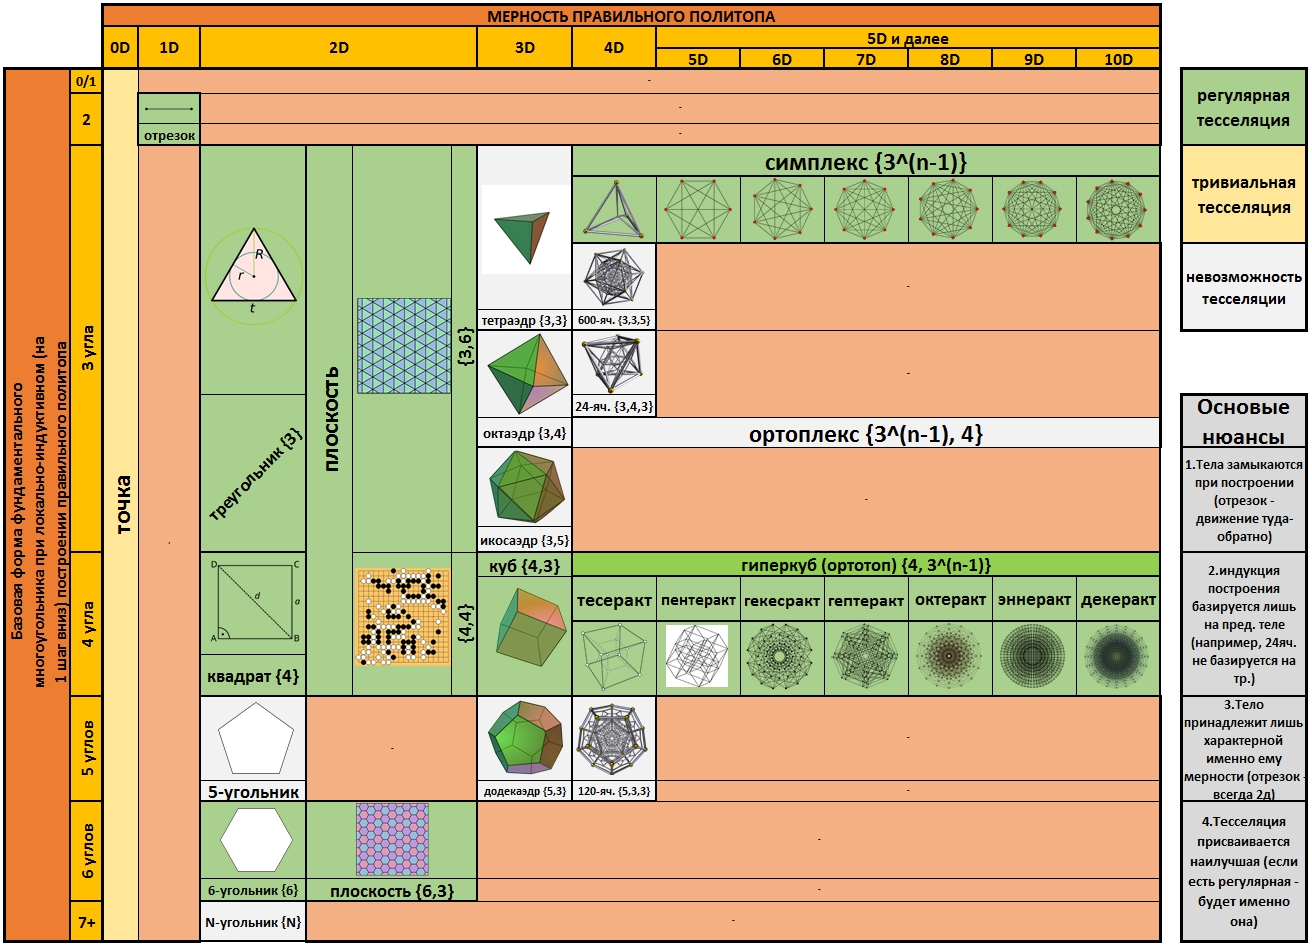
\includegraphics[width=1\textwidth]{СвваПравильныхПолитопов.jpg}
    \caption{Табличка свойств многомерных платоновых (правильных) политопов}
\end{figure}

\section{Анализ}

Подробный анализ и разбор каждого тела, метод построения, развертки. Возврат к многомерным пазлам из начала. Диаграмма Шлегея и символ Шлефли. Доказательство несуществования большего числа политопов в каждой мерности, чем ей присущего. Тесселяции. 

\section{Упражнения для навигации по табличке}

\chapter{Геометрическая визуализация метода авто-доказательств алгебраческих Теорем с помощью гипер-кубоида}

\section{Примеры}

Эквиваленты утверждения из кванторов! Предел, $X = D(f) \Leftrightarrow \forall x \in D(f) \to \nexists x \notin D(f)$  \\
Сжатие гипер-кубоида до гипер-призмы (можно ли схлопнуть до нескольких призм, скленных с несколькими гипперкубоидами - например, призма+прямоугольник?) \\
Обход проблемы через НЕсхлопывание гипер-кубоида в гипер-призму?.. (но задачка классификации все равно интеерсная - решить!)\\
Посчитать число возможных гипер-призм по числу выделенных направлений гипер-кубоида

\section{Упражнения: доказать разные Теоремы с помощью Метода}

\chapter{Теория Групп}

\section{Аксиомы Группы}

\section{Абелева группа}

\section{Упражнения}

Взять из диалога с Гвенью

\section{Аксиомы Морфизмов}

\section{Упражнения}

\section{Теоремы: Упражнения и доказательства}

\section{Повторные Упражнения из начала документа, но уже с точки зрения Теории Групп}

\chapter{Прочие структуры Уналга (Универсальной или Общей Алгебры)}

\section{Полугруппа}

\section{Модоид}

\section{Кольцо}

\section{Кольцо с единицей}

\section{Поле}

\begin{minipage}[t]{\linewidth}
    \centering
    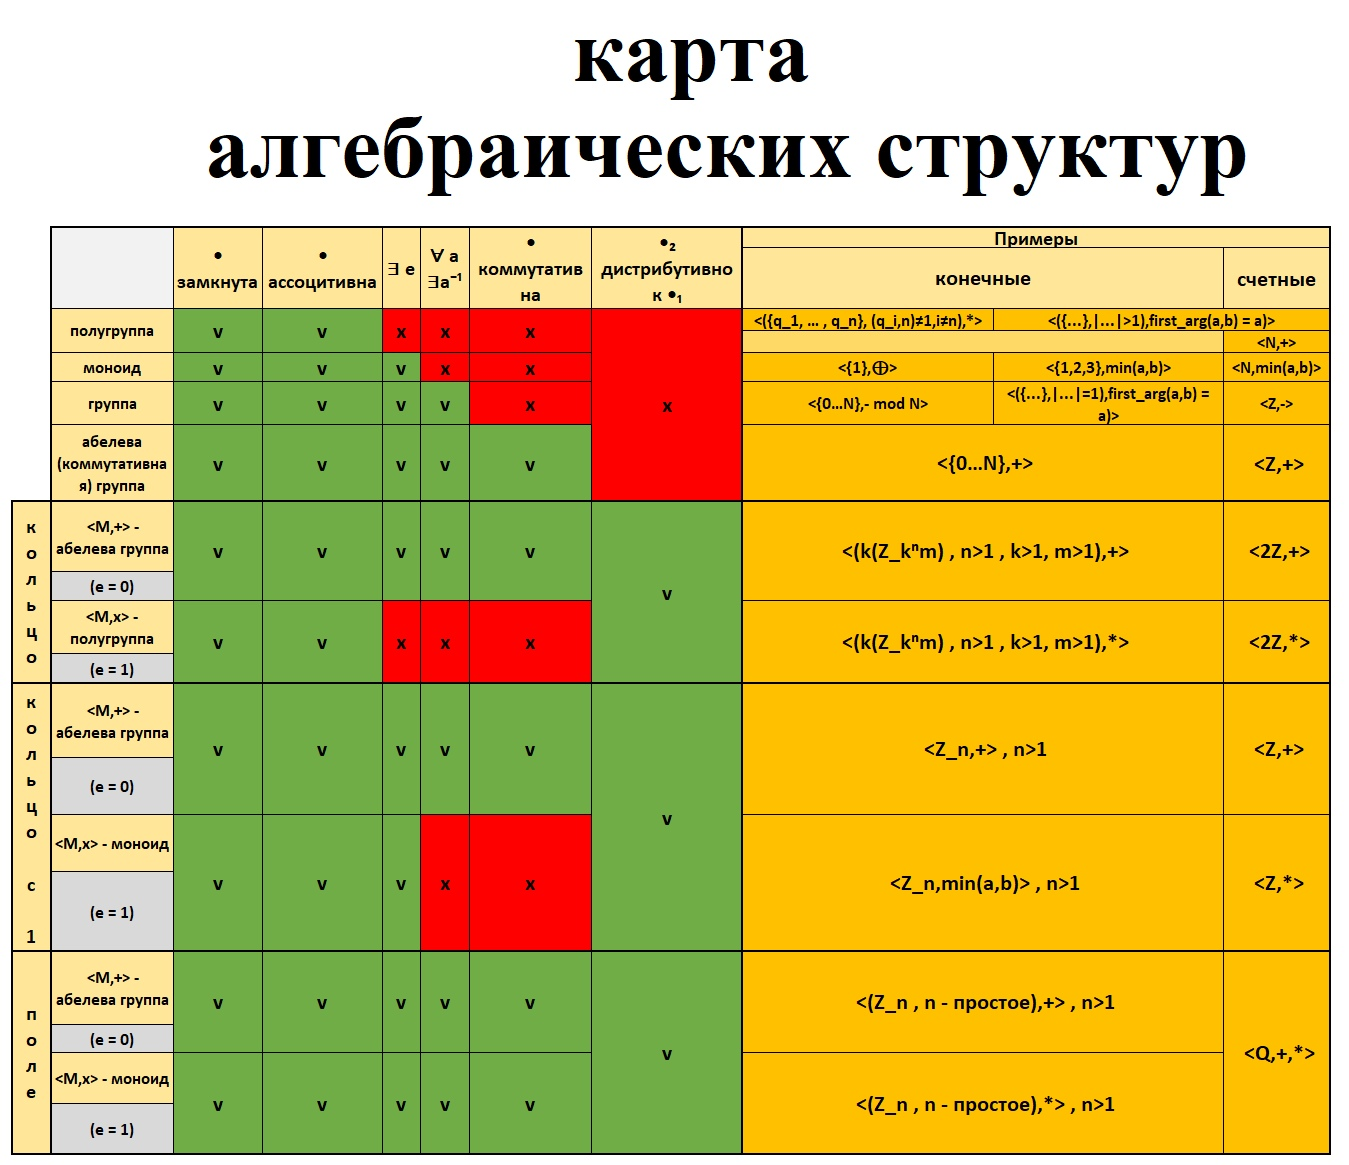
\includegraphics[width=0.8\textwidth]{Уналг.jpg}
    \captionof{figure}{Табличка структур Уналга}
\end{minipage}

\section{Разбор таблички и примеров}

\chapter{Группы Ли}

\chapter{Диаграмма Кокстера-Дынкина}

\chapter{Ответы на все упражнения}

\chapter{Глоссарий}

\end{document}